\documentclass[preprint,12pt,aps,pra,showkeys,amsmath,amssymb,superscriptaddress,floatfix]{revtex4-2}
\usepackage[T1]{fontenc}
\usepackage[utf8]{inputenc}
\usepackage{amsmath,amssymb,amsthm,mathtools,mathrsfs}
\usepackage{microtype,booktabs,enumitem}
\usepackage{xcolor,tikz,etoolbox}
\usepackage[skins,breakable]{tcolorbox}
\usepackage{needspace}
% Keep diagram geometry independent of REVTeX preprint body spacing.
\AtBeginEnvironment{tikzpicture}{\linespread{1}\selectfont}
\usetikzlibrary{arrows.meta,positioning,calc,fit,decorations.pathreplacing}
\usepackage{graphicx}
\usepackage{hyperref}

\definecolor{MMBlue}{RGB}{0,82,155}
\definecolor{MMOrange}{RGB}{200,80,0}
\tikzset{
 mmnode/.style={draw=MMBlue,rounded corners=2pt,fill=MMBlue!4,align=left,execute at begin node={\raggedright},text width=5cm,font=\fontsize{10}{12}\selectfont,inner sep=6pt},
 mmimport/.style={mmnode,draw=black!65,fill=black!4},
 mmcandidate/.style={mmnode,draw=MMOrange,dashed,fill=MMOrange!5},
 mmrejected/.style={mmnode,draw=black,densely dotted,fill=black!8},
 mmproof/.style={->,thick,MMBlue},
 mmflow/.style={->,semithick,black!70},
 mmrepair/.style={->,dashed,thick,MMOrange},
 mmcandidatearrow/.style={->,dashed,semithick,MMOrange},
 mmnote/.style={font=\scriptsize,fill=white,inner sep=2pt,align=center}}

\usepackage[section]{placeins}
\setlength{\emergencystretch}{3em}
\setlist{itemsep=3pt,topsep=4pt}
\newtheorem{theorem}{Theorem}[section]
\newtheorem{proposition}[theorem]{Proposition}
\newtheorem{lemma}[theorem]{Lemma}
\newtheorem{corollary}[theorem]{Corollary}
\theoremstyle{definition}
\newtheorem{definition}[theorem]{Definition}
\newtheorem{example}[theorem]{Example}
\theoremstyle{remark}
\newtheorem{remark}[theorem]{Remark}
% Avoid isolated statement headings and single-line paragraph fragments.
\BeforeBeginEnvironment{theorem}{\Needspace{6\baselineskip}}
\BeforeBeginEnvironment{definition}{\Needspace{5\baselineskip}}
\BeforeBeginEnvironment{proposition}{\Needspace{5\baselineskip}}
\BeforeBeginEnvironment{lemma}{\Needspace{5\baselineskip}}
\BeforeBeginEnvironment{corollary}{\Needspace{5\baselineskip}}
\clubpenalty=5000
\widowpenalty=5000
\newcommand{\R}{\mathbb R}\newcommand{\Z}{\mathbb Z}\newcommand{\N}{\mathbb N}
\newcommand{\Pa}{\operatorname{Pa}}\newcommand{\Desc}{\operatorname{Desc}}
\newcommand{\cl}{\operatorname{cl}}\newcommand{\cost}{\operatorname{cost}}
\newcommand{\status}{\operatorname{status}}
% Faculty cards: a visual rail groups the five faculties within one agent.
% The rail has no arrowhead and does not represent a proof dependency.
\newcommand{\mmfacultybadge}[1]{%
 \node[circle,draw=MMBlue,line width=1pt,fill=white,
 minimum size=7mm,inner sep=0pt,font=\sffamily\small\bfseries,text=MMBlue]
 at ([xshift=15pt,yshift=-15pt]frame.north west) {#1};}
\newcommand{\mmfacultyrail}{%
 \draw[MMBlue!80,line width=1pt]
 ([xshift=15pt,yshift=2pt]frame.north west)--
 ([xshift=15pt,yshift=-2pt]frame.south west);}
\newtcolorbox{mmfacultybox}[2]{enhanced,breakable,
 colback=MMBlue!4,colframe=MMBlue!4,boxrule=0pt,arc=3pt,
 left=39pt,right=9pt,top=4pt,bottom=4pt,
 before skip=2pt,after skip=2pt,
 fontupper=\small\linespread{1.1}\selectfont,
 overlay unbroken={\mmfacultyrail\mmfacultybadge{#1}},
 overlay first={\mmfacultyrail\mmfacultybadge{#1}},
 overlay middle={\mmfacultyrail},overlay last={\mmfacultyrail}}
\newcommand{\mmfaculty}[3]{%
 \begin{mmfacultybox}{#1}{#2}
 {\sffamily\bfseries\color{MMBlue}#2}\par\smallskip #3
 \end{mmfacultybox}}
\newcommand{\agent}[9]{%
 \Needspace{8\baselineskip}
 \subsubsection{#1}
 \noindent\textbf{Object.} #2\par
 \noindent\textbf{Role.} #3\par\smallskip
 \mmfaculty{E}{Ego}{#4}
 \mmfaculty{M}{Memory}{#5}
 \mmfaculty{I}{Intellect}{#6}
 \mmfaculty{S}{Sense}{#7}
 \mmfaculty{A}{Action}{#8}
 \smallskip\noindent #9\par}

\usepackage{longtable,array,calc}
\providecommand{\tightlist}{\setlength{\itemsep}{2pt}\setlength{\parskip}{0pt}}
\makeatletter
\def\frontmatter@abstract@produce{\par\addvspace{\frontmatter@preabstractspace}%
\begingroup\prep@absbox\unvbox\absbox\post@absbox\endgroup
\addvspace{\frontmatter@postabstractspace}}
\makeatother
\newcommand{\field}[2]{\par\smallskip\noindent\textbf{#1.} #2\par}
\setlength{\emergencystretch}{5em}
\AtBeginEnvironment{verbatim}{\small\linespread{1.0}\selectfont}


\hypersetup{colorlinks=true,linkcolor=MMBlue,urlcolor=MMBlue,pdfauthor={Dibakar Sigdel}}

\begin{document}

\title{Rank--Nullity Theorem\\[4pt]\large An End-to-End Meta-Math Walkthrough}

\author{Dibakar Sigdel}

\affiliation{Mindverse Computing LLC, Lynnwood, WA 98087, USA}

\date{October 2026}

\begin{abstract}

A complete authored walkthrough of rank--nullity theorem, with explicit
mathematical contracts, local verification gates, and reusable exports.
The report presents the target theorem, declared imports, a dependency
graph, five-faculty node contracts, a continuous proof, a worked
example, and a hypothesis-repair audit. It is an authored mathematical
exposition, not a deployed-agent transcript or a formal proof-assistant
certificate.

\end{abstract}\maketitle\linespread{1.12}\selectfont

\noindent\textbf{LA-01 / Linear Algebra / Report v1}

\section{Target and import contract}

\begin{theorem}

For a linear map \(T:V\to W\) with finite-dimensional \(V\), prove
\(\dim V=\dim\ker T+\dim\operatorname{im}T\).

\end{theorem}

\subsection{Foundations and permitted imports}

All vector spaces are over one field F. V is finite-dimensional; W need
not be. Import basis extension in a finite-dimensional vector space, and
the definitions of kernel, image, linear independence, and span. The
zero-dimensional cases use an empty basis.

\clearpage\section{Node interaction workflow}

\begin{center}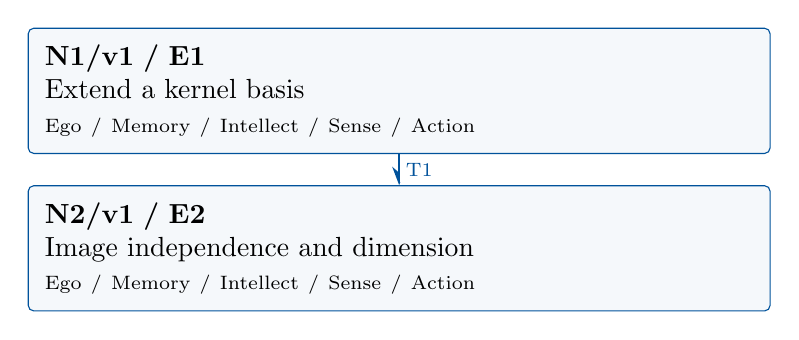
\begin{tikzpicture}[>=Stealth,x=1cm,y=1cm]

\node[mmnode,text width=9cm,minimum height=1.25cm] (N1) at (0,0.0) {\textbf{N1/v1 / E1}\\Extend a kernel basis\\{\scriptsize Ego / Memory / Intellect / Sense / Action}};

\node[mmnode,text width=9cm,minimum height=1.25cm] (N2) at (0,-2.0) {\textbf{N2/v1 / E2}\\Image independence and dimension\\{\scriptsize Ego / Memory / Intellect / Sense / Action}};

\draw[mmproof] (N1.south) -- node[mmnote,right] {T1} (N2.north);

\end{tikzpicture}\end{center}

Each box is one mathematical agent containing all five faculties. Blue
arrows carry the versioned exports listed below. The layout gives a
reading order; only drawn arrows assert dependencies. Diagnostic repair
is separate from the proof DAG.

\subsection{Versioned evidence-transfer ledger}

\begingroup\small\linespread{1.05}\selectfont

\Needspace{5\baselineskip}\field{T1: N1/E1/v1 to N2}{The images \(Tv_{1},\ldots ,Tv_r\) span the image.}

\field{Receiving activity}{N2: Image independence and dimension}

\field{Compatibility}{Use the same mathematical objects and hypotheses as the source export.
Receiving contract: Extended domain basis; prior exports E1/v1}

\endgroup

\clearpage\section{Agent roles and five-faculty activities}\begingroup\small\linespread{1.05}\selectfont\setlist{itemsep=1pt,topsep=2pt}

\subsection{N1/v1: Extend a kernel basis}

\field{Object and role}{Complete the basis in the domain, not the codomain.}

\field{Inputs}{T linear; \(u_{1},\ldots ,u_k\) basis of kerT; foundational imports
stated in §1}

\mmfaculty{E}{Ego}{Own E1/v1: The images \(Tv_{1},\ldots ,Tv_r\) span the image.}

\mmfaculty{M}{Memory}{Retain T linear; \(u_{1},\ldots ,u_k\) basis of kerT; foundational
imports stated in §1; keep their assumptions and versions attached.}

\mmfaculty{I}{Intellect}{Complete the basis in the domain, not the codomain.}

\mmfaculty{S}{Sense}{The added basis vectors must complement the whole kernel.}

\mmfaculty{A}{Action}{Carry out the numbered deductions and publish E1/v1 together with its
hypotheses and proof location.}

\smallskip\noindent\textbf{Numbered mathematical activities}

\begin{enumerate}[label=N1.\arabic*,leftmargin=3.4em]

\item Choose a basis \(u_{1},\ldots ,u_k\) of ker T and extend it to
\(u_{1},\ldots ,u_k,v_{1},\ldots ,v_r\) of V.

\item Thus \(\operatorname{dim} V=k+r\).

\item For any \(x\in V\) write \(x=\sum a_i\) \(u_i+\sum b_j\) \(v_j\).

\item ApplyingT yields \(Tx=\sum b_jTv_j\) because every \(u_i\) lies in the
kernel.

\item Hence the vectors \(Tv_j\) span im T.

\end{enumerate}

\field{Export E1/v1}{The images \(Tv_{1},\ldots ,Tv_r\) span the image.}

\field{Acceptance gate}{The added basis vectors must complement the whole kernel. Publish only
after checking every displayed deduction.}

\field{Targeted repair}{If the check fails, revise N1: The added basis vectors must complement
the whole kernel. Recheck dependent nodes N2.}

\clearpage

\subsection{N2/v1: Image independence and dimension}

\field{Object and role}{Pull a zero combination back to the kernel.}

\field{Inputs}{Extended domain basis; prior exports E1/v1}

\mmfaculty{E}{Ego}{Own E2/v1: Rank--nullity with no finiteness requirement on W.}

\mmfaculty{M}{Memory}{Retain Extended domain basis; prior exports E1/v1; keep their
assumptions and versions attached.}

\mmfaculty{I}{Intellect}{Pull a zero combination back to the kernel.}

\mmfaculty{S}{Sense}{A spanning list alone cannot be counted as a basis.}

\mmfaculty{A}{Action}{Carry out the numbered deductions and publish E2/v1 together with its
hypotheses and proof location.}

\smallskip\noindent\textbf{Numbered mathematical activities}

\begin{enumerate}[label=N2.\arabic*,leftmargin=3.4em]

\item If \(\sum b_jTv_j=0\) then \(\sum b_jv_j\) lies inkerT, so equals
\(\sum a_i\) \(u_i\).

\item Independence of the extended basis forces all \(b_j\) and \(a_i\) zero.

\item Thus \(Tv_j\) are independent and form a basis ofimT.

\item Therefore \(\dim\operatorname{im} T=r\) and
\(\operatorname{dim} V=k+r=\dim\ker T+\dim\operatorname{im} T\).

\item If \(r=0\) this is the empty image basis; if \(k=0\) it states injective
maps preserve domain dimension.

\end{enumerate}

\field{Export E2/v1}{Rank--nullity with no finiteness requirement on W.}

\field{Acceptance gate}{A spanning list alone cannot be counted as a basis. Publish only after
checking every displayed deduction.}

\field{Targeted repair}{If the check fails, revise N2: A spanning list alone cannot be counted
as a basis. Withhold this terminal result until its gate passes.}

\endgroup\clearpage\section{Continuous mathematical proof}\label{sec:proof}

Read these steps in order as one proof; the diagram is optional.
Numbered activities identify the specific constructions and deductions
owned by each node.

\subsection{§4.N1 --- Extend a kernel
basis}\label{n1-extend-a-kernel-basis}

\begin{enumerate}
\def\labelenumi{\arabic{enumi}.}
\item
  Choose a basis \(u_{1},\ldots ,u_k\) of ker T and extend it to
  \(u_{1},\ldots ,u_k,v_{1},\ldots ,v_r\) of V.
\item
  Thus \(\operatorname{dim} V=k+r\).
\item
  For any \(x\in V\) write \(x=\sum a_i\) \(u_i+\sum b_j\) \(v_j\).
\item
  ApplyingT yields \(Tx=\sum b_jTv_j\) because every \(u_i\) lies in the
  kernel.
\item
  Hence the vectors \(Tv_j\) span im T.
\end{enumerate}

\subsection{§4.N2 --- Image independence and
dimension}\label{n2-image-independence-and-dimension}

\begin{enumerate}
\def\labelenumi{\arabic{enumi}.}
\item
  If \(\sum b_jTv_j=0\) then \(\sum b_jv_j\) lies inkerT, so equals
  \(\sum a_i\) \(u_i\).
\item
  Independence of the extended basis forces all \(b_j\) and \(a_i\)
  zero.
\item
  Thus \(Tv_j\) are independent and form a basis ofimT.
\item
  Therefore \(\dim\operatorname{im} T=r\) and
  \(\operatorname{dim} V=k+r=\dim\ker T+\dim\operatorname{im} T\).
\item
  If \(r=0\) this is the empty image basis; if \(k=0\) it states
  injective maps preserve domain dimension.
\end{enumerate}

\hfill$\square$

\section{Worked orchestration}

For \(T:R^{3}\to R^{2}\), \(T(x,y,z)=(x+y,z)\), the kernel has
\(basis(1,-1,0)\). Extend by (0,1,0),(0,0,1); their images are
(1,0),(0,1). Thus \(3=1+2\), and the proof visibly constructs the image
basis.

\subsection{Boundary and hypothesis audit}

The numerical formula uses finite dimensions. With an
infinite-dimensional domain one needs cardinal-dimension statements and
appropriate basis principles; subtracting ``infinite rank'' from
``infinite dimension'' is not valid arithmetic. Sense keeps this
studio's finite-dimensional input contract.

\section{Illustrative failure and repair}

The following is an authored diagnostic scenario. Changed assumptions
define a new contract; they do not retroactively prove the original
statement.

\subsection{Failure and correction}
This is an authored teaching trace, not a recorded agent run.

\begin{enumerate}
\def\labelenumi{\arabic{enumi}.}
\tightlist
\item
  \textbf{Ego \(\to\) Memory:} register the §1 theorem, imports, and
  requested exports before beginning the proof.
\item
  \textbf{Intellect \(\to\) Action:} choose the bridges in §3 and carry
  out the numbered activities in §4; transmit only established E-exports
  along the §2 DAG.
\item
  \textbf{Sense \(\to\) responsible node:} test the specific
  boundary/failure in §5 and the node's individual audit. A failing
  candidate is withheld; downstream nodes may not use it.
\item
  \textbf{Memory + Intellect:} identify whether the error is an omitted
  condition, an invalid inference, or an attempted extension beyond the
  theorem. Restore the exact contract or explicitly state a different
  one.
\item
  \textbf{Action:} redo the affected mathematical activity using the
  repaired condition or inference. Recheck consuming nodes, rather than
  feeding their conclusions back as premises.
\item
  \textbf{Ego:} publish only the supported export with its assumptions
  and proof location. A hypothetical revised export is v2; the written
  proof here is the v1 exposition, not a claim that this repair was
  executed.
\end{enumerate}

\subsection{Hypothesis boundary}
The numerical formula uses finite dimensions. With an
infinite-dimensional domain one needs cardinal-dimension statements and
appropriate basis principles; subtracting ``infinite rank'' from
``infinite dimension'' is not valid arithmetic. Sense keeps this
studio's finite-dimensional input contract.

\subsection{Version and recheck}
Treat any changed assumption as a new contract. Recheck the revised
export and all of its descendants. A backward diagnostic never
establishes an earlier theorem. This is an authored teaching trace, not
an execution log.

\par\medskip\begingroup\small\linespread{1.0}\selectfont\noindent\textbf{Provenance.} This authored proof is complete relative to its declared imports. Reuse
each export with its assumptions, proof, and version. The original
Markdown remains available for comparison.
\par\endgroup

\end{document}
